\documentclass[11pt]{article}
\usepackage{fullpage}
\usepackage{graphicx}
\usepackage{float}
\usepackage{tikz}
\usetikzlibrary{matrix,calc}
%opening
\title{\textbf{Homework 1}}
\author{Adam Sumner \\ ECE 429}
\date{September 21st, 2015}

\begin{document}

\maketitle

\section{Explain the Following Terminologies Briefly}

\begin{itemize}
	\item \textbf{Moore's Law} - The observation that the number of transistors in dense integrated circuits has doubled approximately every two years. Named after Gordan E. Moore
	\item \textbf{Feature Size} - The minimum dimension of a transistor that can be reliably built
	\item \textbf{VLSI Design for Power} - Discipline of design that aims to reduce power dissipations while maintaining adequate throughput rate
	\item \textbf{VLSI Design for Manufacturing} - Discipline of design that aims to produce a product in a timely manner with sufficient yield to be profitable
	\item \textbf{ASIC} - Application-Specific Integrated Circuit. An integrated circuit customized for a particular use, rather than general-purpose use
	\item \textbf{Logical Synthesis} - Process by which an abstract from of circuit behavior (usually represented at RTL) is turned into a design implementation
	\item \textbf{Physical Synthesis} - Step in the design cycle that converts circuit representations of components into geometric representations of shapes which, when they are manufactured in their corresponding layers, will ensure the correct functionality
	\item \textbf{Dynamic Power and Leakage Power} - The power consumed during the switching of a transistor, and the power lost to leakage current of transistors
	\item \textbf{Conduction Band} - The lowest range of vacant electronic states. Determines conductivity of the solid
	\item \textbf{Valence Band} - The highest range of electron energies in which electrons are normally present at absolute zero. Determines conductivity of the solid
	\item \textbf{Velocity Saturation} - Sate of a semiconductor when the carrier velocity reaches a maximum value
	\item \textbf{Subthreshold Conduction} - The current between the source and drain of a MOSFET when the transistor is in the subthreshold region
	\item \textbf{Hot Carriers} - Electrons (holes) in a solid-state electronic device that gains sufficient kinetic energy to overcome a potential barrier in order to break an interface state
	\item \textbf{MOSFET Operation Regions} - Three separate modes of a MOSFET depending on the voltage at the terminals: Cutoff, Triode, and Saturation
\end{itemize}

\section{Exercise 1.5}
\begin{figure}[H]
\centering
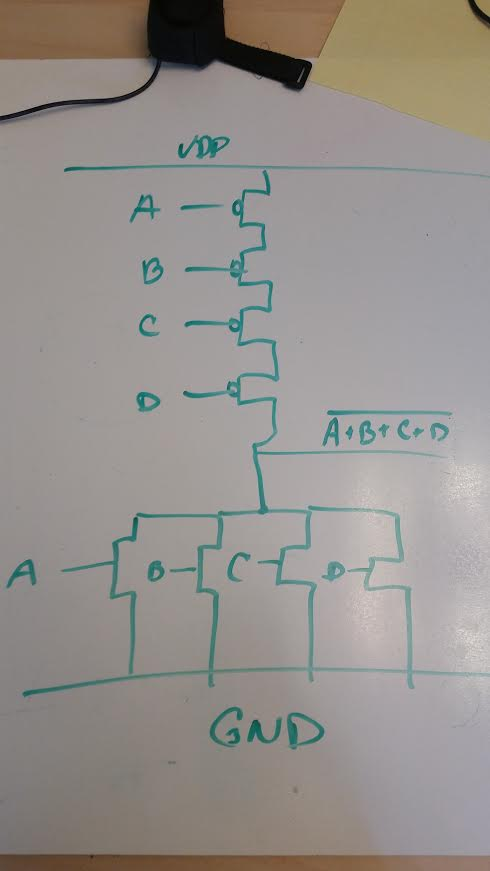
\includegraphics[width=0.5\linewidth]{1-5.jpg}
\caption{4 Input NOR Gate}
\label{fig:1.5}
\end{figure}

\section{Exercise 1.3}
a)
\begin{figure}[H]
\centering
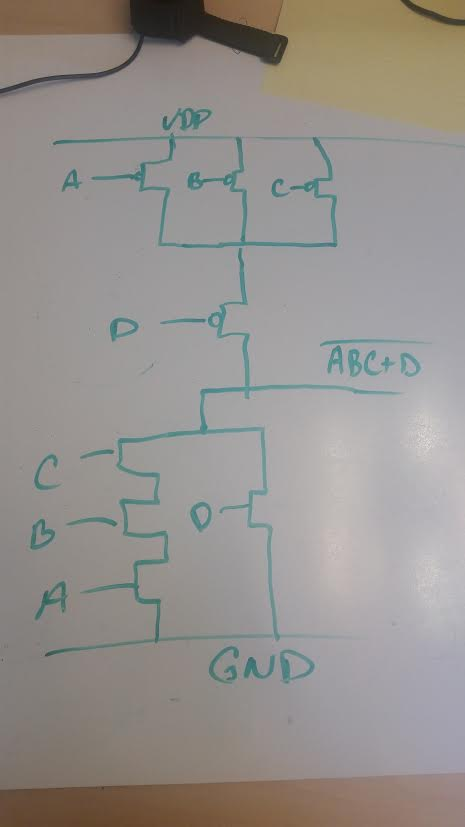
\includegraphics[width=0.5\linewidth]{1-6a}
\caption{$\overline{ABC+D}$}
\label{fig:1.6a}
\end{figure}
b)
\begin{figure}[H]
\centering
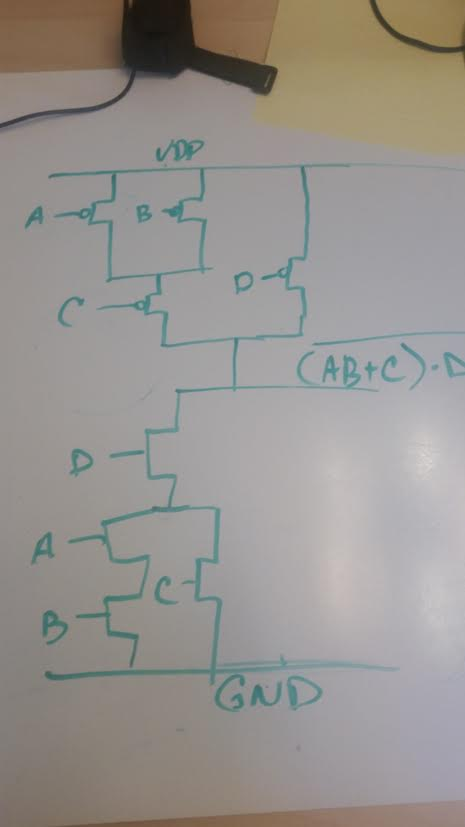
\includegraphics[width=0.5\linewidth]{1-6b}
\caption{$\overline{(AB+C)\cdot D}$}
\label{fig:1-6b}
\end{figure}
c)
\begin{figure}[H]
\centering
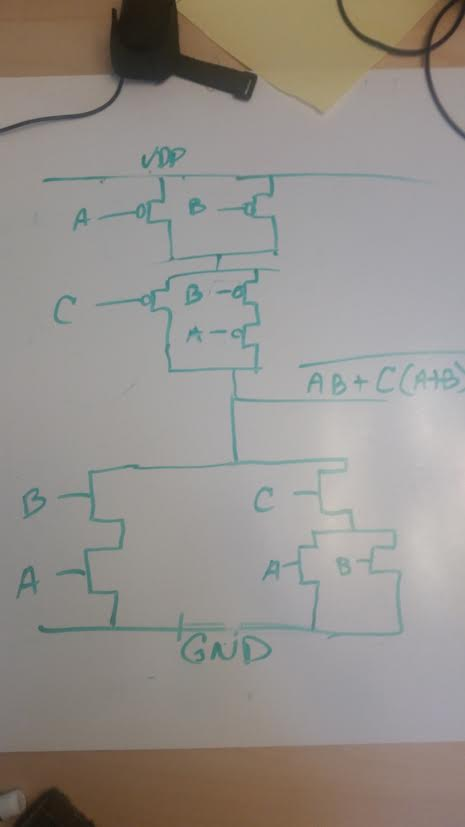
\includegraphics[width=0.5\linewidth]{1-6c}
\caption{$\overline{AB+C(A+B)}$}
\label{fig:1-6c}
\end{figure}
\section{Exercise 1.10}
\begin{figure}[H]
\centering
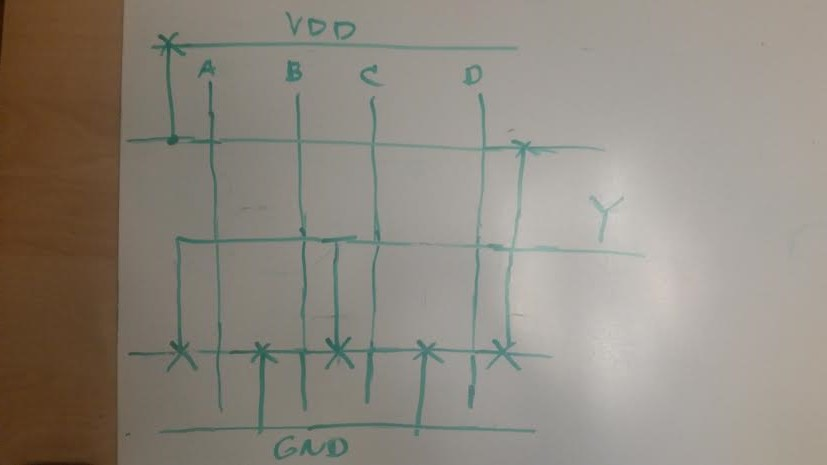
\includegraphics[width=1\linewidth]{1-10}
\caption{Stick Diagram for 4 Input NOR Gate}
\label{fig:1-10}
\end{figure}
\section{Exercise 2.2}

\section{Exercise 2.3}
\section{Exercise 2.7}
\section{Exercise 2.9}
\section{Light Switch Design}
Truth Table \\
\begin{tabular}{|c|c|c|c|}
	\hline
	A & B & C & F\\ \hline
	0 & 0 & 0 & 0 \\ \hline
	0 & 0 & 1 & 1 \\ \hline
	0 & 1 & 1 & 0 \\ \hline
	0 & 1 & 0 & 1 \\ \hline
	1 & 0 & 0 & 1 \\ \hline
	1 & 0 & 1 & 0 \\ \hline
	1 & 1 & 1 & 1 \\ \hline
	1 & 1 & 0 & 0 \\ \hline
\end{tabular}

Karnaugh Map
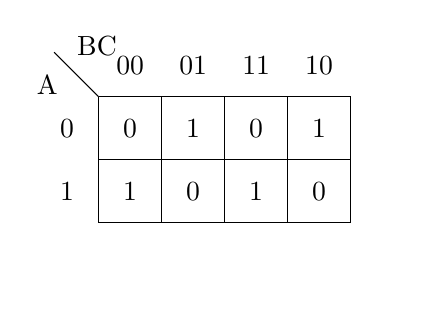
\begin{tikzpicture}[baseline=(current bounding box.north),scale=0.8]
\draw (0,0) grid (4,2);
\draw (0,2) -- node [pos=0.7,above right,anchor=south west] {BC} node [pos=0.7,below left,anchor=north east] {A} ++(135:1);
%
\matrix (mapa) [matrix of nodes,
column sep={0.8cm,between origins},
row sep={0.8cm,between origins},
every node/.style={minimum size=0.3mm},
anchor=4.center,
ampersand replacement=\&] at (0.5,0.5)
{
	\& |(c00)| 00         \& |(c01)| 01         \& |(c11)| 11         \& |(c10)| 10         \& |(cf)| \phantom{00} \\
	|(r00)| 0             \& |(0)|  0 \& |(1)|  1 \& |(3)|  0 \& |(2)|  1 \&                     \\
	|(r01)| 1             \& |(4)|  1 \& |(5)|  0 \& |(7)|  1 \& |(6)|  0 \&                     \\
	|(rf) | \phantom{00}  \&                    \&                    \&                    \&                    \&                     \\
};
%
	\end{tikzpicture}
\\
a)
	$$F = AB'C'+A'B'C+ABC+ABC'$$
	
\begin{figure}[H]
\centering
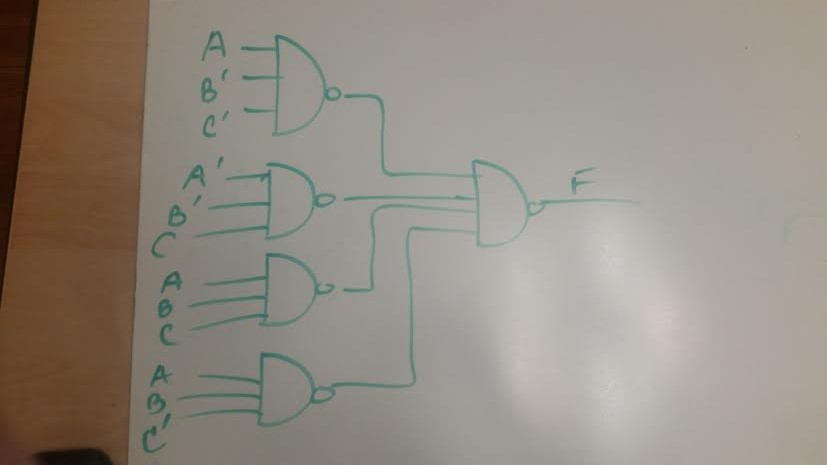
\includegraphics[width=1\linewidth]{nand}
\caption{NAND Gate Implementation}
\label{fig:nand}
\end{figure}
~\\	
b) $$F = (A+B+C)(A+B'+C')(A'+B+C')(A'+B'+C)$$
\begin{figure}[H]
\centering
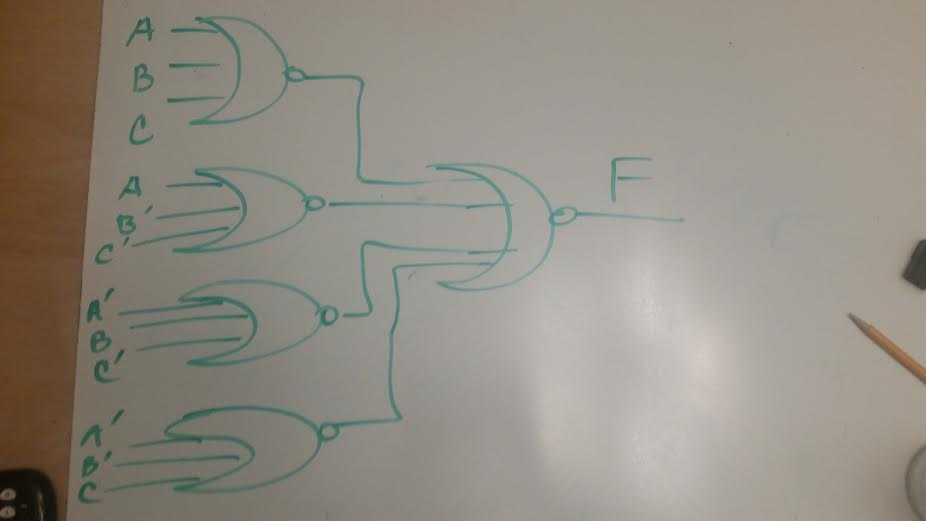
\includegraphics[width=1\linewidth]{nor}
\caption{NOR Gate Implementation}
\label{fig:nor}
\end{figure}

\section{CMOS Compound Gate}
\end{document}
